\section{Verification}
\label{sec:verification}

This chapter evaluates the performance and learning progression og the Deep Q-network
(DQN)-based pokemon battle agent over three iterations. The objective of this analysis
is to validate the effectiveness of the chosen algorithm and whether we have achieved
the desired results based on our reqirements. Performance is assessed through empirical
training results, including average rewards and win rates.

\subsection{Methodology}
Over the 2 Poke-env iterations, the verification process was conducted using the same hyperparameters
but using different formats of the pokemon battle environment.
The first iteration used a single battle format with randomly selected pokemon each
episode, while the second iteration was trained using the VGC 2025 regulation G format.
Each version of the agent, was evaluated over a series of training episodes, and data
was collected for:
\begin{itemize}
    \item Average reward per interval of 10 episodes
    \item Win rate per interval of 10 episodes.
\end{itemize}

\subsubsection{Self-play vs Heuristic Opponents}
All iterations were trained using self-play. In self-play, the agent competes against a copy of itself, allowing it to 
continually adapt and improve its strategies. This approach encourages the development of stronger policies, as the agent 
must learn to counter its own tactics rather than relying on one single strategy. 
A quirk of self-play is that it often leads to a cyclical arms race, where the agent alternates between exploiting and adapting
to its own weaknesses. This has been shown to be an effective method when it comes to training agents in a competitive environment \cite{pmlr-v119-bai20a} like
Pokemon battles. In contrast, training against a heuristic or rule-based opponent might result in the agent overfitting to
a specific strategy, limiting its ability to generalize its own strategies.

\subsection{Results and analysis}
\subsubsection{Iteration 1 - Baseline model}
The first iteration exhibited very fluctuating performance, with a relativly shallow
state representation. Although the agent was capable of learning some degree of a control
policy, its reward curve was very erratic and lacked consistency.
\begin{itemize}
    \item The average reward fluctuated significantly, generally ranging between -10 and +5
          indicating the agent struggled to consistently achieve positive outcomes.
    \item Our Agents winrate hovered around 0.4 to 0.6, which isn't generally bad, it's almost a 50\% winrate
          and shows that it performed marginally better with random teams, but still with no clear upward trend.
\end{itemize}
This indicated that while the agent was learning, it was not effectivly generalizing
information across different battle scenarios, largely due to shallow state information.

\begin{figure}[H]
    \centering
    \includegraphics[width=\textwidth]{assets/Iteration-1-graphs.png}
    \caption{Iteration 1 - Baseline model trained over 1000 episodes}
    \label{fig:iteration-1-graphs}
\end{figure}

\subsubsection{Iteration 2 - Enhanced model}
In the second iteration, the agent was restructured to support:
\begin{itemize}
    \item A more complex battle environment.
    \item More modular hyperparameters, allwing for more fine-tunning.
    \item A bigger Q-network, to account for the increased complexity.
\end{itemize}
This meant the improvements to the second iteration resulted in a smoother reward
distribution, altough still noisy, which is typical for reinforcement learning. The variance
is now centered closer to 0, and positive spikes are more frequent. The win rate
had become more stable, despite some episode by episode variation
and was now more consistently above 0.5 with several peaks reacing about 0.8 or 1.0.
Scalablity has also improved significantly. the agent was able to train over 30000 episodes
compared to the just 1000 episodes in the first iteration, without crashing or instability.

Notably, while the average reward trend was still noisy, the longer training horizon
and improved reward shaping, allowed the agent to learn more stable strategies over time.

\begin{figure}[H]
    \centering
    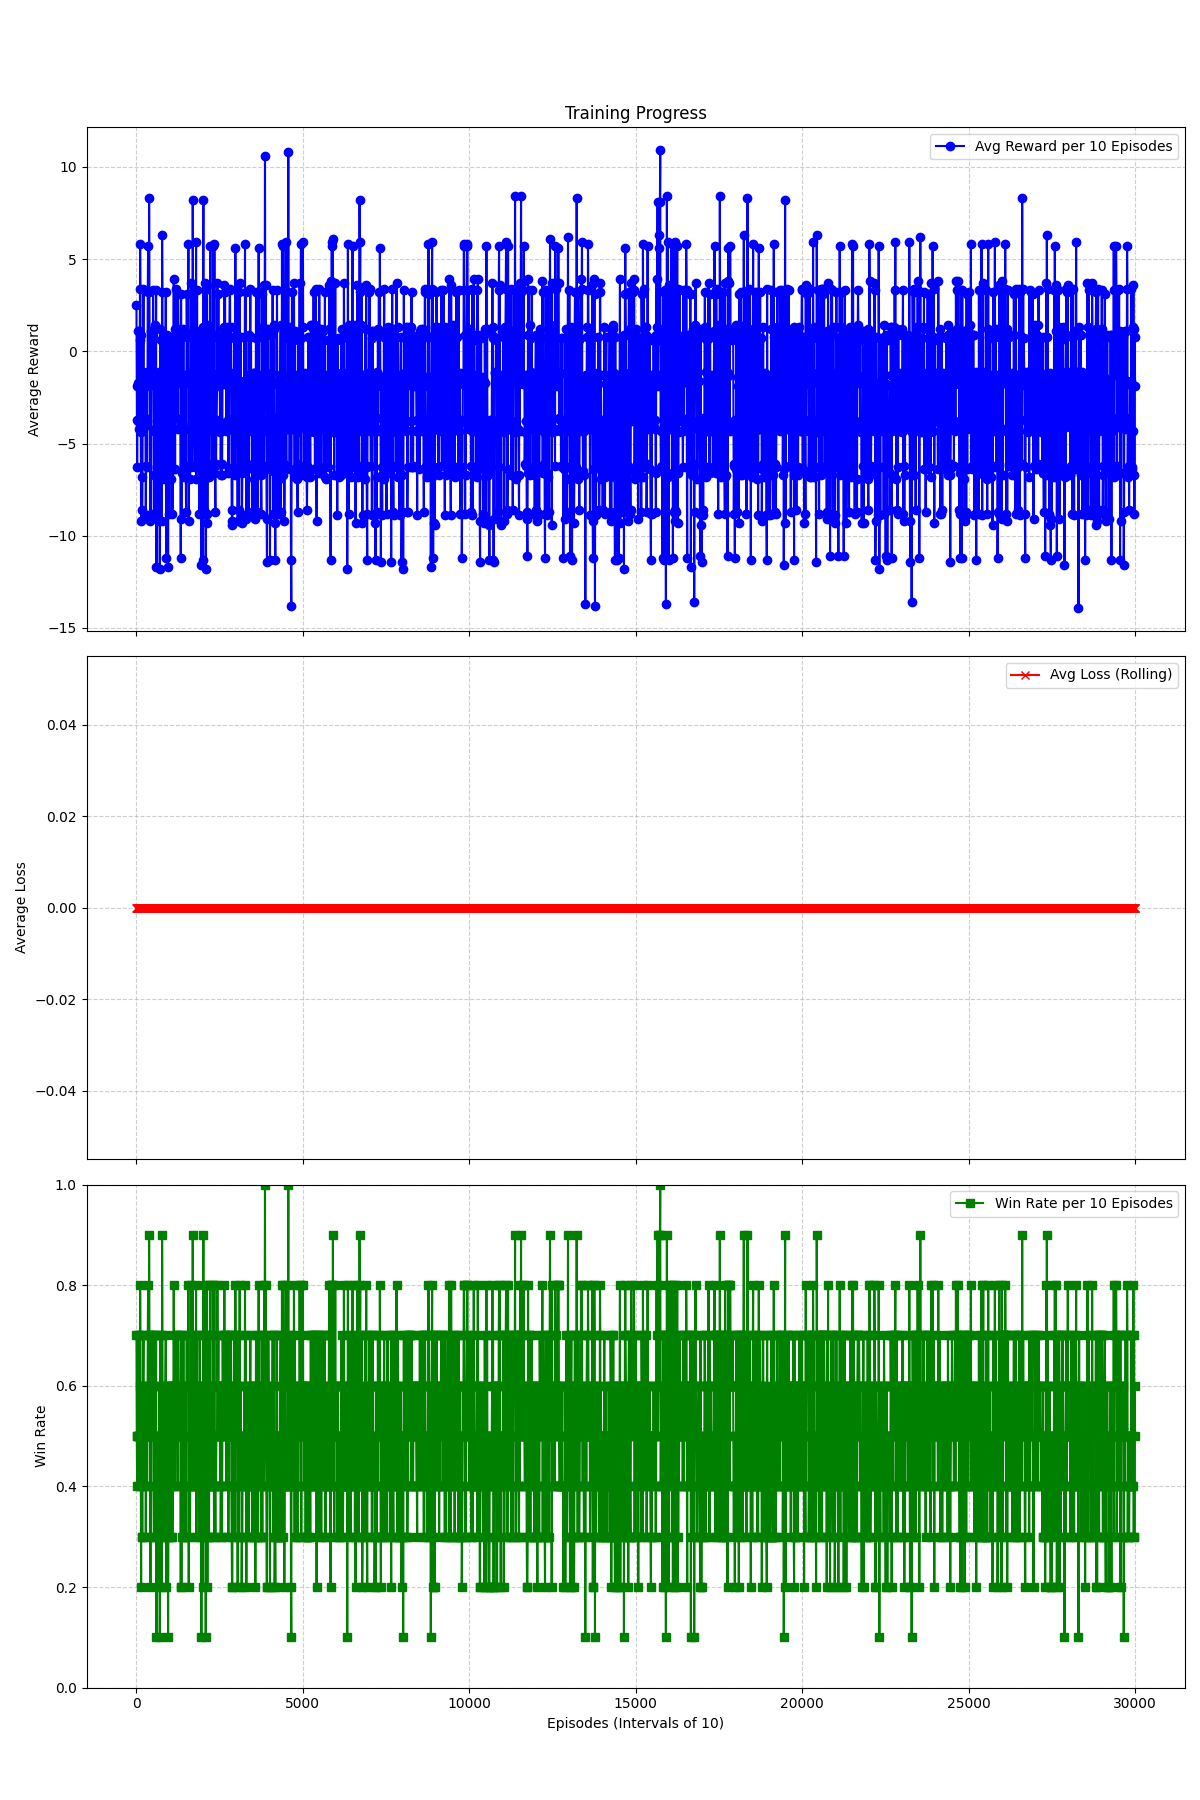
\includegraphics[width=\textwidth]{assets/Iteration-2-graphs.png}
    \caption{Iteration 2 - Enhanced model trained over 30000 episodes}
    \label{fig:iteration-2-graphs}
\end{figure}

\subsubsection{Iteration 3 - Custom environment}
The third iteration used the custom environment and thus had slightly different training conditions compared to the previous iterations.
The custom environment focused its rewards on whether the agent won or lost. For that reason only the rewards are depicted in the graph (see figure \ref{fig:iteration-3-graph}).
The graph depicts the reward the agent received per episode as well as the moving average. A reward of +1 indicates a win and a reward of -1 indicates a loss.

The graph shows that the agent is learning, however it is learning slowly. The moving average tends to hover near +1 or -1, alternating roughly every 1000 episodes.
This behavior is expected when training with self-play. The alternating moving average shows that the player agent learned to beat its opponent, but then the opponent 
agent adapted to the strategy and started to beat the player agent, thus creating a cyclical arms race. 

There are some smooth sections on the graph around episodes 6000 and 7500. These points indicate that the algorithm reached a temporary convergence towards
a stronger policy network, however due to further exploration the agent learned to counter these strategies as well.

An improvement not shown by the graph is stability. In earlier iterations, the agent struggled to train for extended periods of time, but with the new environment
it was able to run 100.000+ episodes without crashing or collapsing. It was not entirely stable, as in rare instances the agent would run into a scenario where it
had no valid actions according to its action mask. This is likely just an implementation error that can be fixed over time, but it tells us that the agent could
potentially train indefinitely if that was desired. 

In the future, more work could be done to make the rewards more detailed in order to shape the models learning capabilites. Rewards could be given for using
super effective moves or knocking out opposing Pokemon.

\begin{figure}[H]
    \centering
    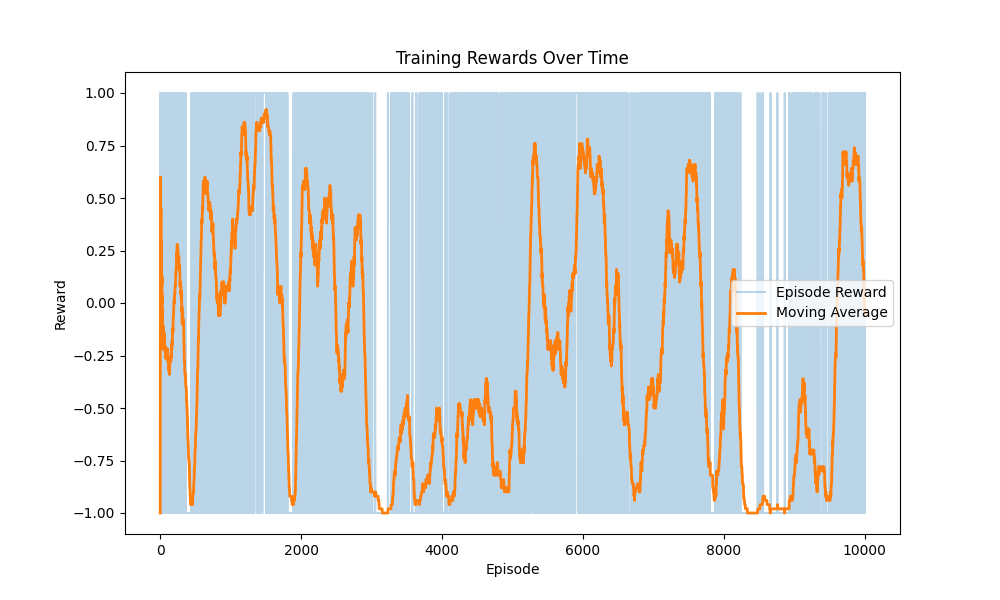
\includegraphics[width=\textwidth]{assets/iteration-3-10k-rewards.png}
    \caption{Iteration 3 - Custom environment over 10000 episodes}
    \label{fig:iteration-3-graph}
\end{figure}

\subsection{Improvements}
The improvements between iterations, can be attributed to several factors:
\begin{itemize}
    \item Expanded state space: Going from a state space of 92 features in the first iteration
          to 128 features in the second iteration, allowed the agent to capture more complex information
          about the environment, leading to better decision making.
    \item Replay buffer: Iteration 2's structured implementation of the replay buffer, improved
          learning consistency and sample efficiency.
    \item Reward design: By incorporating more intermediate rewards (e.g., for knocking out enemies or preserving HP),
          the agent receives more meaningful feedback per action, leading to smoother learning curves.
    \item Network Depth: A deeper DQN enabled our model to better capture complex patterns in the data.
\end{itemize}

A general improvement that could be added to all iterations would be the addition of periodic tests against older iterations of the model.
Since self-play tends to fluctuate in performance depending on which agent is countering which strategy it could provide great value, if 
every 1000 episodes, the agent plays against its initial model from before its current training session. This would help keep track of 
absolute improvements rather than just its relative performance to itself in self-play.
